%% -*- coding: utf-8; -*-

% Use 'digital' option to enable back references. This option is recommended for digital pdf version
\documentclass[phd,american,digital]{thesispuc}%english thesis
%\documentclass[mscr,american]{thesispuc}%english dissertation
%\documentclass[phd,brazilian]{thesispuc}%tese em portugês
%\documentclass[msc,brazilian]{thesispuc}%disseretação em portuguŝ


%%%
%%% Additional Packages
%%%
\usepackage{tabularx}
\usepackage{multirow}
\usepackage{multicol}
\usepackage{colortbl}
\usepackage[%
    dvipsnames,
    svgnames,
    x11names,
    fixpdftex,
    table
]{xcolor}
\usepackage{numprint}
\usepackage{textcomp}
\usepackage{booktabs}
\usepackage{amsmath}
\usepackage{enumitem}
\usepackage{amssymb}
% ABNT reference style package. The current style is the alphabetical order, if you need
% change to citation order, change in the line above 'alf' to 'num', also at the end replace
% bibliographystyle with the commented version.
\usepackage[alf,bibjustif,abnt-emphasize=bf]{abntex2cite}
%\usepackage{tikz}
%\usepackage[linesnumbered, ruled, vlined]{algorithm2e}
%\usepackage{pgfplots,pgfplotstable} 
%\usepackage{array}

%% numprint 
\npthousandsep{.}
\npdecimalsign{,}

%% ThesisPUC option
%\tablesmode{fig} %% [nada, fig, tab ou figtab]
%\algoritmsmode{none} %% [none ou use] %% Default is [use]
%\codesmode{none} %% [none ou use] %% Default is [use]
%\abreviationsmode{none} %% [none ou use] %% Default is [use]

% \makeatletter  \renewcommand\@biblabel[1]{#1}  \makeatother

%%%
%%% Counters
%%%

%% uncomment and change for other depth values
\setcounter{tocdepth}{1}
%\setcounter{lofdepth}{3}
%\setcounter{lotdepth}{3}
%\setcounter{secnumdepth}{3}

%%%
%%% Misc.
%%%

\usecolour{true}


%%%
%%% Titulos
%%%

\author{Felipe Vieira Cortes}
\authorR{Cortes,Felipe V.} % full name

\advisor{Roberto Ierusalimschy}{Prof.} %Name LastName
\advisorR{Ierusalimschy, Roberto} %LastName, Name
% If the advisor's department is different from author's department, uncomment the next line and type the correct name and acronym of advisor's institution.
%\advisorInst{institution name}{acronym}

%\coadvisor{Otávio da Fonseca Martins Gomes}{Dr.}
%\coadvisorR{da Fonseca Martins Gomes, Otávio}
%\coadvisorInst{Centro de Tecnologia Mineral}{CETEM/MCTI}

\title{An alternative formalization of reference typing} %title in portuguese

\titleuk{An alternative formalization of reference typing} %title in english

%%\subtitulo{Aqui vai o subtitulo caso precise}

\day{11}
\month{March}
\year{2023}

\city{Rio de Janeiro}
\CDD{004} 
\department{Informática}
\program{Informática}
\school{Pós-Graduação em Informática}
\university{Pontifícia Universidade Católica do Rio de Janeiro}
\uni{PUC-Rio}


%%%
%%% Jury
%%%

\jury{%
  \jurymember{Roberto Ierusalimschy}{Prof.}
    {Departamento de Informática}{PUC-Rio}
  % \jurymember{Waldemar Celes Filho}{Prof.}
  %   {Departamento de Informática}{PUC-Rio}
}


%%%
%%% Personal Resume
%%%

\resume{%
% If it fit in one line use this command:
% \makebox[\textwidth][s]{Graduated in computer science by the Pontifícia Universidade Católica do Rio de Janeiro.}%
Graduated in computer science by the Pontifícia Universidade Católica do Rio de Janeiro.
% If not just type your resume without any special command 
}

%%%
%%% Acknowledgment (REMINDER TO SCHOLARSHIP STUDENTS. Do not forget to thank the agencies that supported your work.)
%%%
% \acknowledgment{%
% \noindent To my adviser Professor Marcelo Gattass for the stimulus and partnership
% to carry out this work.
% \bigskip

% \noindent To CNPq and PUC-Rio, for the aids granted, without which this work does not
% could have been accomplished.
% \bigskip

% \noindent \textbf{For students contemplated with any CAPES scholarship, whose defense occurred as of 04 September 2018 leave the following passage:} 

% \noindent This study was financed in part by the Coordenação de Aperfeiçoamento de Pessoal
% de Nível Superior - Brasil (CAPES) - Finance Code 001.
% }


%%%
%%% Catalog prekeywords
%%%

\catalogprekeywords{%
  \catalogprekey{Informática}%
}

%%%
%%% Keywords - Don't use % at the end of /key dfinition
%%%

\keywords{%
  \key{Type References}
  \key{Programming Languages}
  \key{Formalization}
}

\keywordsuk{%
  \key{Type References}
  \key{Programming Languages}
  \key{Formalization}
}

%%%
%%% Abstract
%%%

\abstract{%
A tipagem de referencia eh ...
}

\abstractuk{%
Reference Typing is a ... }

%%%
%%% Dedication
%%%

% \dedication{%
%   To my parents, for their support\\
% and encouragement.
% }

%%%
%%% Epigraph
%%%

\epigraph{%
  My beautifull epigraph
}
\epigraphauthor{Wassily Kandinsky}
\epigraphbook{Regards sur le passé}


\begin{document}
  % -*- coding: utf-8; -*-

\chapter{Introduction}

So, to start with, could you provide me with more details about your research idea? What specific area in the field of programming languages are you interested in? What problem or question would you like your research to address?

Sure. I'll provide you with more details about our research idea. I will present you some background information so we can formulate an enthralling laconic research proposal for our target audience.

I am interested in Typing Mutable References. The main reference for the problem my research adresses is the Software Foundations series by Benjamin C. Pierce. The first two volumes, "Logical Foundations" and "Programming Language Foundations" gives a solid understanding of "functional programming, basic concepts of logic, computer-assisted theorem proving, and Coq." and also "the theory of programming languages, including operational semantics and static type systems." respectively. More specifically, the chapter "References" contains a very interesting implementation of mutable references in a Simply Typed Lambda Calculus (STLC) language that we take as an inspiration for condcting our study aroud typing mutable references.


The main idea behind our study is to
    - propose a different approach for the syntax definition of terms inside a Simply Typed Lambda Calculus (STLC) language.
    - redefine the operational semantics comprising our new term definition
    - Check if the standard type safety properties still hold (progress and preservation theorems).
    - Analyse both solutions (canonical and research) comparing simplicity, reasoning, understanding and proof implementations.


Naturally, when introducing mutable references in a language definition, we would consider the following terms (as described in the book Programming Language Foundations, chapter References):

```coq
(** *** Terms *)

(** Besides variables, abstractions, applications,
    natural-number-related terms, and [unit], we need four more sorts
    of terms in order to handle mutable references:

        t ::= ...              Terms
            | ref t              allocation
            | !t                 dereference
            | t := t             assignment
            | l                  location
*)

Inductive tm  : Type :=
    (* STLC with numbers: *)
    | tm_var    : string -> tm
    | tm_app    : tm -> tm -> tm
    | tm_abs    : string -> ty -> tm -> tm
    | tm_const  : nat -> tm
    | tm_succ    : tm -> tm
    | tm_pred    : tm -> tm
    | tm_mult    : tm -> tm -> tm
    | tm_if0  : tm -> tm -> tm -> tm
    (* New terms: *)
    | tm_unit   : tm
    | tm_ref    : tm -> tm
    | tm_deref  : tm -> tm
    | tm_assign : tm -> tm -> tm
    | tm_loc    : nat -> tm.
```


% \begin{figure}
% \centering
% 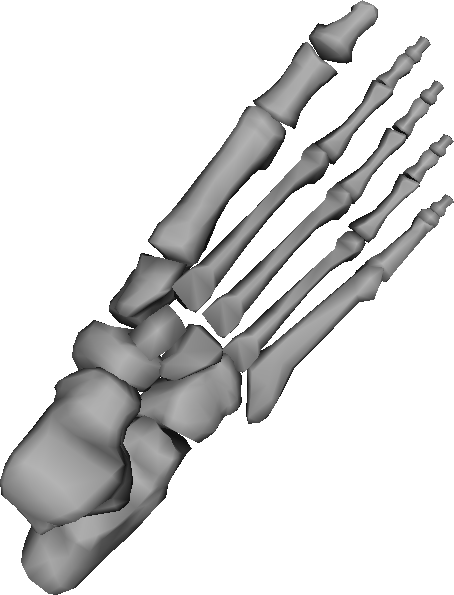
\includegraphics[width=0.45\textwidth]{pictures/image01.png}
% 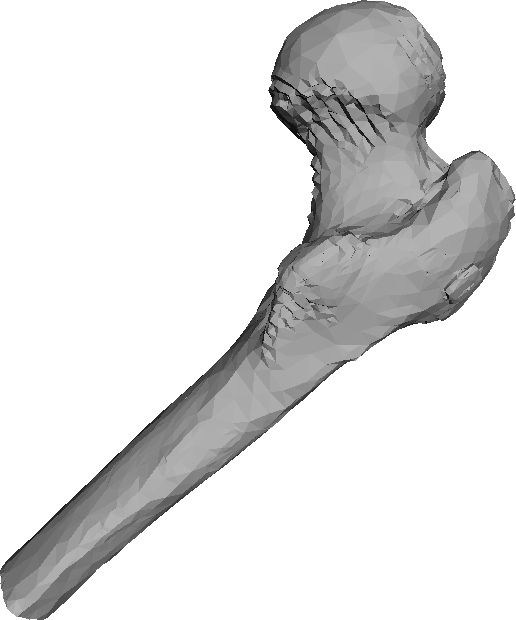
\includegraphics[width=0.45\textwidth]{pictures/image02.png}
% \caption{Meshes generated from medical data. Data obtained from the AIM$@$SHAPE Shape Repository \cite{AIMSHAPE}}
% \label{fig:example}
% \end{figure}


This document is structured as follows. In Chapter~\ref{cha:Previous Work} we present some previous work relevant to our problem. In Chapter~\ref{cha:Proposal} we explain our proposal. In Chapter~\ref{cha:Results} we show our results. Finally, in Chapter~\ref{cha:Conclusion} we present our conclusion and future work.


 % introduction
  % -*- coding: utf-8; -*-

\chapter{Previous Work}
\label{cha:Previous Work}

Early smoothing methods tried to minimize... In the figure \ref{subfig:pictures/image01.png} we see...

\subimages{A set of three subfigures:
(a) describes the first subfigure;
(b) describes the second subfigure;
(c) describes the third subfigure.}{55}
{
 \subimage[Bamboo-pile Vertically Inserted Position]{.45}{pictures/image01.png}
 \subimage[Bamboo-pile Normal Inserted Position]{.45}{pictures/image02.png}\\
 \subimage[bamboo-pile Inserted 45° angle]{.45}{example-image}
}
\newpage
\csubimages{A set of six subfigures in two pages.}{55}
{
 \subimage[Bamboo-pile Vertically Inserted Position]{.45}{pictures/image01.png}
 \subimage[Bamboo-pile Normal Inserted Position]{.45}{pictures/image02.png}\\
 \subimage[bamboo-pile Inserted 45° angle]{.45}{example-image}
}
\ssubimages{A set of six subfigures in two pages.(Continuation)}{55}
{
 \subimage[Bamboo-pile Vertically Inserted Position]{.45}{pictures/image01.png}
 \subimage[Bamboo-pile Normal Inserted Position]{.45}{pictures/image02.png}\\
 \subimage[bamboo-pile Inserted 45° angle]{.45}{example-image}
} % previous work
  % -*- coding: utf-8; -*-
\chapter{Proposal}
\label{cha:Proposal}

Equation example 1:

\begin{equation}
\begin{split}
\min_u \int_{x_i\in X}\int_{x_j\in X} q_{ij} u_i u_j da da + \int_{x_i\in X}||x' - x_i|| u_i da \\
s.t. \ \ \ u\in[0,1] \ \ \land  \ \ \int_{x_i\in X}u da = a_0,
\end{split}
\end{equation}

Equation exmaple 2:

\begin{equation}
\begin{split}
\min_{\mathbf{u}} \alpha \mathbf{u}^T \mathbf{A}^T \mathbf{Q} \mathbf{A} \mathbf{u} +  \beta \mathbf{d}^T a' \mathbf{A} \mathbf{u} + \gamma \mathbf{u}^T \mathbf{G}^T \mathbf{G} \mathbf{u} + \delta\mathbf{f}^T a' \mathbf{A} \mathbf{u} \\
s.t. \ \ \ \mathbf{0} \leq \mathbf{u} \leq \mathbf{1} \land \mathbf{a}^T\mathbf{u}=a_0.
\end{split}
\end{equation}

Equation example 3:
\begin{align}
\mathbf{G}=(g_{ij}) = \left\lbrace
\begin{array}{ll}
\sum_{f_k\in N_f(f_i)} l_{ik} & i=j\\
-l_{ij} & e_{ij}\in E\\
0 & \text{otherwise}
\end{array}
\right.
\end{align}

\lstinputlisting[label=mean,title={Mean Filter},caption={Mean Filter},language=R]{codes/mean.R}

%% Poruguese algorithm
%\begin{algorithm}
%\DontPrintSemicolon
%\Entrada{Malha e quantidade de pontos a ser amostrado}
%\Saida{Pontos amostrados na malha}
%\BlankLine
%\emph{Crie um vetor de números randômicos entre $[0,1]$ com a %quantidade de pontos a ser amostrada e ordene-o}\;
%\emph{Calcule a área total dos triângulos da malha}\;
%\For{$i=0$ \KwTo numeroDePontos} {
%  \emph{Navegue entre as faces acumulando a sua $\frac{area}{areaTotal}$ até achar a face com valor acumulado $\geqslant$ numerosRandomicos[i]}\;
%  \emph{Pegue um ponto randômico dentro da face utilizando o %método de Turk e adicione no vetor do resultado}\;
%}
%\caption{Escolha das amostras inicias}\label{alg:sampling}
%\end{algorithm}\DecMargin{1em}

%% enlgish algorithm
\begin{algorithm}
\DontPrintSemicolon
\KwIn{Malha e quantidade de pontos a ser amostrado}
\KwOut{Pontos amostrados na malha}
\BlankLine
\emph{Crie um vetor de números randômicos entre $[0,1]$ com a quantidade de pontos a ser amostrada e ordene-o}\;
\emph{Calcule a área total dos triângulos da malha}\;
\For{$i=0$ \KwTo numeroDePontos} {
  \emph{Navegue entre as faces acumulando a sua $\frac{area}{areaTotal}$ até achar a face com valor acumulado $\geqslant$ numerosRandomicos[i]}\;
  \emph{Pegue um ponto randômico dentro da face utilizando o método de Turk e adicione no vetor do resultado}\;
}
\caption{Escolha das amostras inicias}\label{alg:sampling}
\end{algorithm}\DecMargin{1em}







  % -*- coding: utf-8; -*-

\chapter{Results}
\label{cha:Results}

Table example. Table~\ref{tab:res} shows results. 

\begin{table}[!h]
\caption{Results for devil mesh}
\tiny
\begin{center}
\begin{tabular}{ m{1.1cm} m{0.95cm} m{0.95cm} m{0.95cm} m{0.95cm} m{0.95cm} m{0.95cm} m{0.95cm} m{0.95cm} m{0.95cm} } 
 & Mean Vertex Distance & L2 Vertex Based & Mean Quadric & MSAE & L2 Normal Based & Tangential & Mean Discrete Curvature & Area Error & Volume Error\\ 
 \hline 
\cite{FDC03} & 0.061277 & 0.110973 & 0.236219 & 19.697900 & 0.055170 & 0.047678 & 0.090284 & 0.051443 & 0.045645 \\ 
 \cite{JDD03} & 0.001293 & 0.002800 & 0.002289 & 21.237300 & 0.021589 & 0.013026 & 0.087991 & 0.000364 & 0.002621 \\ 
 \cite{SRML07} & 0.001439 & 0.002880 & 0.003540 & 14.043200 & 0.012654 & 0.008911 & 0.055849 & 0.007806 & 0.000582 \\ 
 \cite{ZFAT11} & \cellcolor{blue!25}0.000713 & \cellcolor{blue!25}0.001537 & 0.001824 & 12.171400 & \cellcolor{blue!25}0.009654 & \cellcolor{blue!25}0.005781 & \cellcolor{blue!25}0.054567 & 0.005617 & \cellcolor{blue!25}0.000425 \\ 
 \cite{HS13} & 0.002531 & 0.004560 & 0.007108 & 13.830100 & 0.017459 & 0.010314 & 0.114528 & 0.001686 & 0.001786 \\ 
 \cite{ZDZBL15} & 0.001623 & 0.003079 & 0.005048 & \cellcolor{blue!25}10.454200 & 0.015233 & 0.008054 & 0.094668 & 0.002629 & 0.001326 \\ 
 \cite{YRP16} & 0.000737 & 0.001548 & \cellcolor{blue!25}0.001493 & 16.880800 & 0.014129 & 0.006974 & 0.079952 & \cellcolor{blue!25}0.000209 & 0.002375 \\ 
 Ours & 0.000987 & 0.001902 & 0.002686 & 11.574200 & 0.010632 & 0.006796 & 0.075106 & 0.003970 & 0.000722 \\ 
 \end{tabular}
\end{center}
 \label{tab:res}
\end{table}

\section{Comparison}
  \chapter{Conclusion and future work}
\label{cha:Conclusion}

We proposed an algorithm for triangular mesh denoising with detail preservation...

\lstinputlisting[label=mean2,title={Mean Filter},caption={Mean Filter},language=R]{codes/mean.R}
  %% ...
  \arial
  \bibliographystyle{abnt-alf} % \bibliographystyle{abnt-num}
  \bibliography{main} 
\end{document}
